%% Referee Version
\documentclass[referee,sn-basic]{sn-jnl} % referee option is meant for double line spacing

%% Final Version
%%\documentclass[sn-mathphys-num]{sn-jnl} % Math and Physical Sciences Numbered Reference Style 

%%%% Standard Packages
\usepackage{graphicx}%
\usepackage{multirow}%
\usepackage{amsmath,amssymb,amsfonts}%
\usepackage{amsthm}%
\usepackage{mathrsfs}%
\usepackage[title]{appendix}%
\usepackage{xcolor}%
\usepackage{textcomp}%
\usepackage{manyfoot}%
\usepackage{booktabs}%
\usepackage{algorithm}%
\usepackage{algorithmicx}%
\usepackage{algpseudocode}%
\usepackage{listings}%

\usepackage{physics}% added to use braket notation

%%% To be removed once finished
\newcommand{\todo}[1]{\textcolor{green}{[TODO: #1]}}

\begin{document}

\title[Quantum Circuits Noise Simulation with Reinforcement Learning]{Quantum Circuits Noise Simulation with Reinforcement Learning}

\author*[1,2,4]{\fnm{Simone} \sur{Bordoni}}\email{simone.bordoni@uniroma1.it}

\author[2,4]{\fnm{Andrea} \sur{Papaluca}}\email{andrea.papaluca@anu.edu.au}
\equalcont{These authors contributed equally to this work.}

\author[1,2]{\fnm{Piergiorgio} \sur{Buttarini}}\email{add@email.com}
\equalcont{These authors contributed equally to this work.}

\author[2,5]{\fnm{Alejandro} \sur{Sopena}}\email{add@email.com}
\equalcont{These authors contributed equally to this work.}

\author[2,6]{\fnm{Stefano} \sur{Carrazza}}\email{add@email.com}

\author[1,4]{\fnm{Stefano} \sur{Giagu}}\email{stefano.giagu@uniroma1.it.com}

\affil[1]{\orgdiv{Dep. of Physics}, \orgname{La Sapienza University of Rome}, \orgaddress{\street{Piazzale Aldo Moro 2}, \city{Rome}, \postcode{00185}, \state{Italy}}}

\affil[2]{\orgdiv{Quantum Research Center}, \orgname{Technology Innovation Institute}, \orgaddress{\street{Masdar City}, \city{Abu Dhabi}, \postcode{9639}, \state{United Arab Emirates}}}

\affil[3]{\orgdiv{School of Computing}, \orgname{The Australian National University}, \orgaddress{\street{108 North Rd}, \city{Canberra}, \postcode{2601}, \state{Australia}}}

\affil[4]{\orgdiv{Sez. di Roma}, \orgname{INFN}, \orgaddress{\street{Piazzale Aldo Moro 2}, \city{Rome}, \postcode{00185}, \state{Italy}}}

\affil[5]{\orgdiv{Instituto de Fisica Teorica, UAM/CSIC}, \orgname{Universidad Autonoma de Madrid}, \orgaddress{\street{C. Nicolás Cabrera 13-15}, \city{Madrid}, \postcode{28049}, \state{Spain}}}

\affil[6]{\orgdiv{TIF Lab}, \orgname{Università degli Studi di Milano}, \orgaddress{\street{Via Celoria 16}, \city{Milan}, \postcode{20133}, \state{Italy}}}

\abstract{Quantum computing in the NISQ era requires powerful tools to reduce the gap between simulations and quantum hardware execution. 
In this work, we present a machine learning approach to characterize a noise model and reproduce it during simulations. 
The proposed algorithm is based on reinforcement learning and is meant to be more flexible, in reproducing different models of noise, 
than standard techniques like randomized benchmarking or heuristic noise models. 
We have tested the proposed model both with simulations and on real superconducting qubits. 
We also include two use-case examples. The first is a simulation of noisy circuits to famous quantum algorithms, 
the second is an application to quantum machine learning.}

%%% Improved copylot version
% In the current era of quantum computing, powerful tools are essential to bridge the gap between simulations and quantum hardware execution. 
% This paper introduces a machine learning approach for characterizing a noise model and replicating it during simulations. 
% The proposed algorithm, grounded in reinforcement learning, offers greater flexibility in reproducing various noise models 
% compared to conventional techniques such as randomized benchmarking or heuristic noise models. 
% The model's effectiveness has been validated through simulations and real-world testing on superconducting qubits. 
% Additionally, this paper provides two practical use-case examples: a simulation of noisy circuits applied to renowned quantum algorithms, 
% and an application to quantum machine learning.

\keywords{keyword1, Keyword2, Keyword3, Keyword4}

%%\pacs[JEL Classification]{D8, H51}

%%\pacs[MSC Classification]{35A01, 65L10, 65L12, 65L20, 65L70}

\maketitle
\section{Introduction}
One important unsolved technological questions is whether Noise Intermediate Scale Quantum (NISQ)~\cite{Preskill_2018} computers will be useful 
for practical applications. In fact, quantum computers are expected to offer speedups over classical computers in certain computational 
tasks~\cite{Shor_1997, grover1996fast, Zhong_2020}. 
However, NISQ devices are limited in usability and reliability mainly because of errors due to: gate infidelities, unwanted interactions with the 
environment, thermal relaxation, measurement errors and 
cross-talk~\cite{PhysRevLett.121.090502, doi:10.1146/annurev-conmatphys-031119-050605, PRXQuantum.3.020301, PhysRevB.104.045420, 9355264}. 
Hence, it is widely regarded that near-term quantum advantage will only be achieved through advanced error mitigation 
techniques~\cite{PRXQuantum.2.040326, PhysRevA.105.062404, 10.1145/3352460.3358265, Sopena_2021, PRXQuantum.2.040330} or only with the future generations 
of fault-tolerant quantum devices~\cite{article_knill, PhysRevX.8.021054, PhysRevA.86.032324, Varsamopoulos_2017, bordoni2023}.
Even if no advantage has been proven on NISQ devices, many algorithms have been developed and deployed on this hardware. In particular machine learning 
inspired models has shown encouraging results in the last 
years~\cite{Biamonte_2017, 8939749, Cerezo_2021, egger2023study, particles6010016, Robbiati:2853183, robbiati2022quantum, cruzmartinez2023multivariable}.
In order to study these kind of algorithms it is important to be able to emulate their behavior when executed on imperfect quantum chips. 
In this work we want to develop a model able to learn a hardware specific noise to be used for predictions during circuit simulations. 
This objective is further motivated by the fact that very few techniques of noise modeling or noise prediction are available to this 
date~\cite{zlokapa2020deep, inproceedings_caracterization, PhysRevA.104.062432, Harper_2020}.
In our approach we train an agent with Reinforcement Learning 
(RL)~\cite{sutton2018reinforcement, kaelbling1996reinforcement, wiering2012reinforcement}, in order to add noise channels to reproduce the noise pattern 
of a specific quantum chip. In this way we reduce as much as possible the heuristic assumption on the noise model, 
thus increasing the adaptability and generalization properties of the algorithm.\\

\noindent
This article is structured as follows:\\
In Section~\ref{sec_background} we introduce the basic concepts necessary to understand the proposed algorithm, reinforcement learning and the noise in quantum circuits. \\
In Section~\ref{sec_methodology} we describe in detail the reinforcement learning algorithm, with particular regard to its training and its use for noise prediction. \\
Section~\ref{sec_results} reports the results obtained with the proposed algorithm both on simulations and on real quantum devices, the performance is also compared with other noise predictors. \\
In Section~\ref{sec_applications} we show examples use-cases of the algorithm for quantum machine learning and quantum Fourier transform applications.

%% Improved copylot version
% \section{Introduction}
% The utility of Noise Intermediate Scale Quantum (NISQ)~\cite{Preskill_2018} computers for practical applications remains a significant technological 
% question. Despite the expectation that quantum computers will outperform classical computers in certain computational 
% tasks~\cite{Shor_1997, grover1996fast, Zhong_2020}, the usability and reliability of NISQ devices are hindered by errors. 
% These errors stem from gate infidelities, unwanted environmental interactions, thermal relaxation, measurement errors, and 
% cross-talk~\cite{PhysRevLett.121.090502, doi:10.1146/annurev-conmatphys-031119-050605, PRXQuantum.3.020301, PhysRevB.104.045420, 9355264}. 
% Consequently, it is widely accepted that near-term quantum advantage can only be realized through advanced error mitigation 
% techniques~\cite{PRXQuantum.2.040326, PhysRevA.105.062404, 10.1145/3352460.3358265, Sopena_2021, PRXQuantum.2.040330} or with future generations 
% of fault-tolerant quantum devices~\cite{article_knill, PhysRevX.8.021054, PhysRevA.86.032324, Varsamopoulos_2017, bordoni2023}.

% Despite the lack of proven advantage on NISQ devices, numerous algorithms have been developed and implemented on this hardware. 
% Machine learning-inspired models, in particular, have shown promising results in recent 
% years~\cite{Biamonte_2017, 8939749, Cerezo_2021, egger2023study, particles6010016, Robbiati:2853183, robbiati2022quantum, cruzmartinez2023multivariable}. 
% To study these algorithms, it is crucial to emulate their behavior when executed on imperfect quantum chips. 
% This work aims to develop a model capable of learning hardware-specific noise for use in circuit simulations. 
% This goal is further motivated by the limited availability of noise modeling or noise prediction 
% techniques~\cite{zlokapa2020deep, inproceedings_caracterization, PhysRevA.104.062432, Harper_2020}.

% Our approach employs Reinforcement Learning (RL)~\cite{sutton2018reinforcement, kaelbling1996reinforcement, wiering2012reinforcement} to train an agent 
% to add noise channels that replicate the noise pattern of a specific quantum chip. 
% This method minimizes heuristic assumptions about the noise model, thereby enhancing the adaptability and generalization properties of the algorithm.

% This article is structured as follows:
% Section~\ref{sec_background} introduces the basic concepts necessary to understand the proposed algorithm, reinforcement learning, and noise in quantum circuits.
% Section~\ref{sec_methodology} provides a detailed description of the reinforcement learning algorithm, focusing on its training and use for noise prediction.
% Section~\ref{sec_results} presents the results obtained with the proposed algorithm on both simulations and real quantum devices, and compares its performance with other noise predictors.
% Section~\ref{sec_applications} demonstrates examples of the algorithm's use-cases for quantum machine learning and quantum Fourier transform applications.

\section{Background}\label{sec_background}
This section provides an overview of the essential concepts required to comprehend the proposed noise simulation algorithm. 
Specifically, we will briefly discuss noise in quantum circuits and introduce reinforcement learning.

\subsection{Noise in quantum circuits}
Quantum noise is a crucial challenge faced in quantum circuits, which can significantly impact the expected results of computations on NISQ hardware. 
Qubits are susceptible to various sources of noise, such as environment interaction, spontaneous emission or calibration errors. 
Errors accumulate during the execution of a quantum circuit making the final result less accurate or even completely erroneous. 
Many mathematical tools have been developed in order to describe quantum noise~\cite{PhysRev.121.920, nielsen_chuang_2010, 10.1117/12.2017396}. 
In this work we will model quantum noise using error channels, which are represented as superoperators acting on state density matrices. 
The following list provides a concise overview of the error channels utilized in this study:
\begin{description}
    \item[Depolarizing:] this channel acts uniformly on all possible quantum states. 
    Depolarization refers to the flattening or averaging of the quantum state, making it less distinguishable from other possible states, 
    leading to a loss of coherence and entanglement. Depolarization is typically quantified by a parameter $\lambda$, which represents the probability of an error occurring in the transmission or processing of the state. The depolarizing channel act on a single qubit state $\rho$ as follows:
    \begin{equation*}
    Dep_\lambda(\rho)=(1-\lambda)\rho+\lambda\mathbb{I}.
    \end{equation*}
    
    \item[Amplitude Damping:] this channel models physical processes, occurring on the qubits, that involve energy dissipation or spontaneous emission. The amplitude damping channel describes a decay process where the state $\ket{0}$ is conserved while $\ket{1}$ decays to $\ket{0}$ with probability $\gamma$:
    \begin{equation*}
    Damp(\gamma)\ket{1}=(1-\gamma)\ket{1}+\gamma\ket{0}
    \end{equation*}
    This channel is similar to the thermal relaxation channel but does not take into account the phase decoherence. We decided to use the amplitude damping because, even if less general, it needs a single parameter instead of the three parameters necessary to describe the thermal relaxation. This makes the training of the RL agent easier and less prone to overfitting. Moreover, we have not noticed any significant performance reduction when applying this channel instead of the thermal relaxation during preliminary tests.
    
    \item[Coherent errors:] this kind of errors are unitary and can be represented with single qubit rotation gates ($R_x$, $R_y$, $R_z$). They can arise for several reasons like a wrong calibration, cross-talk, external fields, and residual qubit–qubit interactions~\cite{Cenedese_2023}. For example, when a rotation gate ($R(\theta)$) is applied, a coherent error can introduce an unwanted perturbation in the rotation angle ($R(\theta+\epsilon)$). Because of their different nature, coherent errors can have strong effects on quantum error correction codes~\cite{Greenbaum_2017, Venn_2023, Beale_2018}. On the other hand, as these errors do not destroy quantum information, once identified, they can be corrected~\cite{Cenedese_2023, Kern_2005, Bravyi_2018}.
\end{description}
\noindent
Different noise channels can be combined in order to create complex noise models~\cite{PhysRevA.104.062432, article_model_realistic}. 
The parameters of the channels can be inferred from calibration results or directly from quantum circuits execution like in this work.
In order to obtain a simple modeling of the noise, it is possible to use a technique called Randomized Benchmarking 
(RB)~\cite{Emerson_2005, heinrich2023randomized, 2019npj}.
With RB it is possible to estimate the magnitude of the average error in a set of quantum gates. 
This estimation can be performed in an efficient way, resources required scale polynomially with the number of qubits in the device. 
The general idea behind RB is that of applying sequences of randomly chosen quantum gates of varying length. 
Small errors are thus amplified with the sequence length, and gate quality measures can be extracted from the dependence of the output data on sequence length.
The noise model obtained in this way is unrealistic as all noise sources are projected on the depolarizing channel. 
However, this technique allows to compute a good average gate fidelity and can be used as a basic benchmark for other, more sophisticated, 
noise characterization techniques.

%% Improved copylot version
% \subsection{Noise in quantum circuits}
% Quantum noise is a significant challenge in quantum circuits, 
% which can drastically affect the expected results of computations on NISQ hardware. 
% Qubits are vulnerable to various sources of noise, such as environmental interaction, 
% spontaneous emission, or calibration errors. 
% Errors accumulate during the execution of a quantum circuit, 
% making the final result less accurate or even completely erroneous. 

% Many mathematical tools have been developed to describe quantum noise~\cite{PhysRev.121.920, nielsen_chuang_2010, 10.1117/12.2017396}. 
% In this work, we model quantum noise using error channels, 
% which are represented as superoperators acting on state density matrices. 

% The following list provides a concise overview of the error channels utilized in this study:
% \begin{description}
%     \item[Depolarizing:] This channel acts uniformly on all possible quantum states. 
%     Depolarization refers to the flattening or averaging of the quantum state, 
%     making it less distinguishable from other possible states, 
%     leading to a loss of coherence and entanglement. 
%     Depolarization is typically quantified by a parameter $\lambda$, 
%     which represents the probability of an error occurring in the transmission or processing of the state. 
%     The depolarizing channel act on a single qubit state $\rho$ as follows:
%     \begin{equation*}
%     Dep_\lambda(\rho)=(1-\lambda)\rho+\lambda\mathbb{I}.
%     \end{equation*}
    
%     \item[Amplitude Damping:] This channel models physical processes, 
%     occurring on the qubits, that involve energy dissipation or spontaneous emission. 
%     The amplitude damping channel describes a decay process where the state $\ket{0}$ is conserved 
%     while $\ket{1}$ decays to $\ket{0}$ with probability $\gamma$:
%     \begin{equation*}
%     Damp(\gamma)\ket{1}=(1-\gamma)\ket{1}+\gamma\ket{0}
%     \end{equation*}
%     This channel is similar to the thermal relaxation channel but does not take into account the phase decoherence. 
%     We decided to use the amplitude damping because, even if less general, 
%     it needs a single parameter instead of the three parameters necessary to describe the thermal relaxation. 
%     This makes the training of the RL agent easier and less prone to overfitting. 
%     Moreover, we have not noticed any significant performance reduction 
%     when applying this channel instead of the thermal relaxation during preliminary tests.
    
%     \item[Coherent errors:] This kind of errors are unitary and can be represented with single qubit rotation gates ($R_x$, $R_y$, $R_z$). 
%     They can arise for several reasons like a wrong calibration, cross-talk, external fields, and residual qubit–qubit interactions~\cite{Cenedese_2023}. 
%     For example, when a rotation gate ($R(\theta)$) is applied, a coherent error can introduce an unwanted perturbation in the rotation angle ($R(\theta+\epsilon)$). 
%     Because of their different nature, coherent errors can have strong effects on quantum error correction codes~\cite{Greenbaum_2017, Venn_2023, Beale_2018}. 
%     On the other hand, as these errors do not destroy quantum information, once identified, they can be corrected~\cite{Cenedese_2023, Kern_2005, Bravyi_2018}.
% \end{description}

% Different noise channels can be combined to create complex noise models~\cite{PhysRevA.104.062432, article_model_realistic}. 
% The parameters of the channels can be inferred from calibration results or directly from quantum circuits execution like in this work.
% In order to obtain a simple modeling of the noise, 
% it is possible to use a technique called Randomized Benchmarking (RB)~\cite{Emerson_2005, heinrich2023randomized, 2019npj}.
% With RB, it is possible to estimate the magnitude of the average error in a set of quantum gates. 
% This estimation can be performed in an efficient way, 
% resources required scale polynomially with the number of qubits in the device. 
% The general idea behind RB is that of applying sequences of randomly chosen quantum gates of varying length. 
% Small errors are thus amplified with the sequence length, 
% and gate quality measures can be extracted from the dependence of the output data on sequence length.
% The noise model obtained in this way is unrealistic as all noise sources are projected on the depolarizing channel. 
% However, this technique allows to compute a good average gate fidelity 
% and can be used as a basic benchmark for other, more sophisticated, noise characterization techniques.

\subsection{Reinforcement learning}\label{sec_rl}
In this article we propose to apply Machine Learning (ML) techniques to the problem of noise modeling.
In particular, we have decided to use reinforcement learning that is a powerful paradigm in ML that deals with the training of an agent to make 
optimal decisions in a dynamic environment. From a mathematical perspective a RL algorithm is described as a Markov Decision Process (MDP)~\cite{PUTERMAN1990331}. 
In a MDP the future state depends solely on the current state and action, regardless of the history of previous states and actions. 
MDPs rely on the fundamental concepts of policy, reward functions and discount factors. 
The policy determines the behavior of the agent mapping the states of the environment to actions. 
The reward function assigns a numeric value to state-action pairs, indicating the immediate desirability or cost associated with them. 
The discount factor balances the importance of immediate rewards against future rewards, allowing for consideration of long-term consequences. 
Solving MDPs involves finding an optimal policy that maximizes the expected cumulative reward.
In a RL model the policy is implemented by an artificial Neural Network~\cite{Zou2009} (NN). 
In order to train the NN different episodes of agent-environment interaction are executed. 
At the end of each episode (or batch of episodes) the cumulative reward is computed and is used to update the weights of the NN using the backpropagation 
algorithm~\cite{Rojas1996}.\\
In recent years many different optimization methods have been developed to improve RL convergence and stability during training~\cite{ozalp2020}. 
In our work we have obtained the best results using the Proximal Policy Optimization (PPO)~\cite{schulman2017proximal}. 
This optimization method provides an increased stability by constraining the policy update to a proximity region. 
Moreover PPO is able to handle a continuous action space, necessary to accurately model quantum noise. 
One drawback is its sensitivity to hyperparameters, poorly chosen values can impact convergence and overall performance. 
In order to define and train the algorithm we have used the library \textit{Stable\_Baselines3}~\cite{JMLR:v22:20-1364}. 
This library is built on top of \textit{OpenAI Gym}~\cite{article_gym} which provides a wide range of customizable environments for reinforcement 
learning tasks. Gradient optimization has been performed with \textit{pytorch}~\cite{NEURIPS2019_9015}.

%% Improved copylot version
% In this article, we propose the application of Machine Learning (ML) techniques, 
% specifically reinforcement learning, to the problem of noise modeling. 
% Reinforcement learning is a powerful ML paradigm that trains an agent to make optimal decisions in a dynamic environment. 

% From a mathematical perspective, a reinforcement learning algorithm is described as a Markov Decision Process (MDP)~\cite{PUTERMAN1990331}. 
% In an MDP, the future state depends solely on the current state and action, 
% regardless of the history of previous states and actions. 
% MDPs rely on the fundamental concepts of policy, reward functions, and discount factors. 

% The policy determines the agent's behavior by mapping the states of the environment to actions. 
% The reward function assigns a numeric value to state-action pairs, 
% indicating the immediate desirability or cost associated with them. 
% The discount factor balances the importance of immediate rewards against future rewards, 
% allowing for consideration of long-term consequences. 
% Solving MDPs involves finding an optimal policy that maximizes the expected cumulative reward.

% In a reinforcement learning model, the policy is implemented by an artificial Neural Network (NN)~\cite{Zou2009}. 
% To train the NN, different episodes of agent-environment interaction are executed. 
% At the end of each episode (or batch of episodes), the cumulative reward is computed 
% and used to update the weights of the NN using the backpropagation algorithm~\cite{Rojas1996}.

% Many optimization methods have been developed in recent years to improve reinforcement learning convergence and stability during training~\cite{ozalp2020}. 
% In our work, we have obtained the best results using the Proximal Policy Optimization (PPO)~\cite{schulman2017proximal}. 
% This optimization method provides increased stability by constraining the policy update to a proximity region. 
% Moreover, PPO can handle a continuous action space, which is necessary to accurately model quantum noise. 
% One drawback is its sensitivity to hyperparameters; poorly chosen values can impact convergence and overall performance. 

% To define and train the algorithm, we used the \textit{Stable\_Baselines3} library~\cite{JMLR:v22:20-1364}. 
% This library is built on top of \textit{OpenAI Gym}~\cite{article_gym}, 
% which provides a wide range of customizable environments for reinforcement learning tasks. 
% Gradient optimization was performed with \textit{pytorch}~\cite{NEURIPS2019_9015}.

\section{Algorithm Implementation}\label{sec_methodology}
This section outlines the proposed noise modeling algorithm, 
with a particular emphasis on the training procedure 
and the transformation of quantum circuits into input feature vectors for the neural networks. 
These steps remain consistent whether the algorithm is applied to quantum circuit simulations or real quantum hardware execution. 
For the simulation phase, we utilized \textit{Qibo}~\cite{Efthymiou_2021}, 
an open-source software designed for efficient evaluation of quantum circuits.

\subsection{Training procedure}\label{sec_training}

\begin{algorithm*}
\caption{Training procedure}\label{alg:train}
\begin{algorithmic}
\For{$episode$ in $n\_episodes$}
    \State{$circuit$ = random\_extraction($training\_set$)}
    \For{$moment$ in $circuit$}
        \State{$observation$ = $agent$.make\_observation($circuit$, $moment$)}
        \State{$action$ = $agent$.action($observation$)}
        \State{$circuit$.add\_noise($action$)}
    \EndFor
    \State{$generated\_dm$ = extract\_density\_matrix($circuit$)}
    \State{$reward$ = compute\_reward($generated\_dm$, $ground\_truth\_dm$)}
    \State{$agent$.update\_policy($reward$)}
\EndFor
\end{algorithmic}
\end{algorithm*}

The task of the RL agent is to learn and being able to reproduce a specific noise pattern. This is achieved with the following steps.\\
A non noisy, QCR is given to the agent at the beginning of each episode (random extraction from the training set). For every circuit moment the agent performs an observation of the circuit and makes an action that consists in putting any number of noise channels with a chosen parameter. At the end of an episode the DM of the circuit obtained with this process is computed (generated DM). The generated DM is compared with the real noisy circuit DM (Section~\ref{sec_dataset}), their fidelity is used to compute the final reward and update the weights of the policy NN (Section~\ref{sec_rl}).
After many episodes the agent should learn, in principle, where to put noise channels in a non-noisy circuit in order to reconstruct the DM of the real noisy circuit. 
A summary of this training procedure is reported in Algorithm~\ref{alg:train}. Once trained, the proposed algorithm should be able to generalize to previously unseen circuits to be used to perform realistic noisy simulations.\\

\noindent
Below is reported a description of the main elements of the RL algorithm employed in the training process.
\begin{description}
    \item[Observation:] performing an observation returns the feature vector that is given to the policy NN to decide the next. The observation shape is: 
    $$[\,qubits,\: kernel\_size,\: encoding\_dim\,].$$
    The first and the latter parameter where already described in Section~\ref{sec_dataset}. The $kernel\_size$ parameter has been introduced to make the agent adapt to circuits of different length, and has a similar role to the kernels used in convolutional neural networks~\cite{GU2018354}. The $kernel\_size$ defines a "window" that has the role of limiting how many moments of the circuit the agent can see for each observation. For example, if $kernel\_size=3$ at each step the agent will observe only the current moment, the previous and the next one. The center of the window start from the first moment and slides of a position at each step until the end of the circuit is reached. This implementation is motivated by the heuristic assumption that the noise on a gate is influenced more by the gates that are executed at the same moment or closer in time.

    \item[Policy NN:] this neural network takes as input the current observation and outputs the corresponding action. As the training has been performed with the PPO technique (Section~\ref{sec_rl}) the policy NN is divided into the actor NN (that chooses the action) and the critic NN (that tries to predict the reward). The policy NN has been tuned based on the number of qubits but in general is composed of a first feature extractor composed of a convolutional layer followed by a dense layer. The output of the feature extractor is then passed to the actor and critic NN, both composed of two dense layers. The policy NN has a number of total trainable parameters of the order of $10^4$, this allows a fast training and execution on both GPU and CPU hardware.

    \item[Action:] the output of the policy NN encodes the information regarding the the noise channels added to the circuit at each moment. It can be represented as an array of shape:
    $$[\,qubits, \: noisy\_channels\,].$$
    In this work the possible noise channels are four: depolarizing, amplitude damping and coherent errors $RX$ and $RZ$. For every noise channel the action vector encodes the noise parameter, this parameter is set to zero if no noise channel of that kind is added. For example, in a two qubit circuit, the action:
    \begin{equation*}
    \left[\begin{array}{cccc}
    0.1 & 0 & 0 & 0.2 \\
    0 & 0.05 & 0.3 & 0
    \end{array} \right]
    \end{equation*}
    means that a depolarizing channel with depolarizing probability $0.1$ and a $R_x$ coherent error of rotation angle $0.2$ are added to the first qubit. While a amplitude damping channel with damping probability $0.05$ and a $R_z$ coherent error of rotation angle $0.3$ are added to the second qubit.

    \item[Reward:] it is computed at the end of each episode and is used to update the weights on the policy NN. The reward is related to the distance between the predicted DM and the real noisy circuit DM; the closer they are, the higher is the reward. The distance between the density matrices can be estimated by computing the mean squared error (MSE). MSE can't be used directly as a reward, so we have tried different functional forms. The best results have been obtained using:
    $$reward \,= \,-log(MSE+\epsilon)$$
    where $\epsilon$ is a small parameter that avoids infinite values.
\end{description}

%% Copylot improved version
% \subsection{Training procedure}\label{sec_training}

% \begin{algorithm*}
% \caption{Training procedure}\label{alg:train}
% \begin{algorithmic}
% \For{$episode$ in $n\_episodes$}
%     \State{$circuit$ = random\_extraction($training\_set$)}
%     \For{$moment$ in $circuit$}
%         \State{$observation$ = $agent$.make\_observation($circuit$, $moment$)}
%         \State{$action$ = $agent$.action($observation$)}
%         \State{$circuit$.add\_noise($action$)}
%     \EndFor
%     \State{$generated\_dm$ = extract\_density\_matrix($circuit$)}
%     \State{$reward$ = compute\_reward($generated\_dm$, $ground\_truth\_dm$)}
%     \State{$agent$.update\_policy($reward$)}
% \EndFor
% \end{algorithmic}
% \end{algorithm*}

% The RL agent's task is to learn and reproduce a specific noise pattern. This is achieved through the following steps: 

% 1. A non-noisy Quantum Circuit Representation (QCR) is given to the agent at the beginning of each episode (random extraction from the training set). 
% 2. For every circuit moment, the agent observes the circuit and makes an action, which involves adding any number of noise channels with a chosen parameter. 
% 3. At the end of an episode, the Density Matrix (DM) of the circuit obtained with this process is computed (generated DM). 
% 4. The generated DM is compared with the real noisy circuit DM (Section~\ref{sec_dataset}), and their fidelity is used to compute the final reward and update the weights of the policy Neural Network (NN) (Section~\ref{sec_rl}).

% After many episodes, the agent should learn where to put noise channels in a non-noisy circuit to reconstruct the DM of the real noisy circuit. Algorithm~\ref{alg:train} summarizes this training procedure. Once trained, the proposed algorithm should be able to generalize to previously unseen circuits for realistic noisy simulations.

% Below is a description of the main elements of the RL algorithm employed in the training process:

% \begin{description}
%     \item[Observation:] Performing an observation returns the feature vector given to the policy NN to decide the next action. The observation shape is: 
%     $$[\,qubits,\: kernel\_size,\: encoding\_dim\,].$$
%     The $kernel\_size$ parameter has been introduced to adapt the agent to circuits of different lengths, similar to the kernels used in convolutional neural networks~\cite{GU2018354}. The $kernel\_size$ defines a "window" that limits how many moments of the circuit the agent can see for each observation.

%     \item[Policy NN:] This neural network takes the current observation as input and outputs the corresponding action. The policy NN is divided into the actor NN (that chooses the action) and the critic NN (that tries to predict the reward). The policy NN has a total of approximately $10^4$ trainable parameters, allowing for fast training and execution on both GPU and CPU hardware.

%     \item[Action:] The output of the policy NN encodes the information regarding the noise channels added to the circuit at each moment. It can be represented as an array of shape:
%     $$[\,qubits, \: noisy\_channels\,].$$
%     For every noise channel, the action vector encodes the noise parameter, which is set to zero if no noise channel of that kind is added.

%     \item[Reward:] It is computed at the end of each episode and is used to update the weights on the policy NN. The reward is related to the distance between the predicted DM and the real noisy circuit DM; the closer they are, the higher is the reward. The distance between the density matrices can be estimated by computing the mean squared error (MSE). The best results have been obtained using:
%     $$reward \,= \,-log(MSE+\epsilon)$$
%     where $\epsilon$ is a small parameter that avoids infinite values.
% \end{description}

\subsection{Circuit Representation}
To train the RL agent, we need to represent a quantum circuit as an array that can serve as input for the policy neural network. 
This array is referred to as the Quantum Circuit Representation (QCR). 
Generally, the shape of the QCR is $[\,qubits,\: depth,\: encoding\_dim\,]$, where $encoding\_dim$ depends on the number of primitive gates 
and the number of noise channels. 
The first dimension of the QCR identifies the circuit qubit, while the second dimension identifies the circuit moment. 
The $encoding\_dim$ stores the information of gates and noise channels acting on a specific qubit and circuit moment.\\
The first $n$ entries are set to one in the presence of a single qubit gate, zero otherwise. 
In our work, $n=2$ to encode the presence of an $R_x$ or $R_z$ gate. The $n+1$ entry encodes the presence of a two-qubit gate 
($1$ if a $CZ$ is present, $0$ otherwise). For single qubit circuits, this entry is always set to zero. \\
The $n+2$ entry encodes the rotation angle of single qubit gates, its value is set to zero if no rotation gate is present. 
Rotation angles have been divided by $2\pi$ to set them in the interval $[0,1]$. \\
The remaining entries report the parameters of the noise channels in the following order: Depolarizing channel, Amplitude damping channel, $R_z$ coherent error, and $R_x$ coherent error. 
If no noise channel is present, the respective parameter value is set to zero. \\
Figure~\ref{fig_qcr} provides an example of the QCR of a two-qubit circuit obtained with this procedure.

\begin{figure}
    \centering
    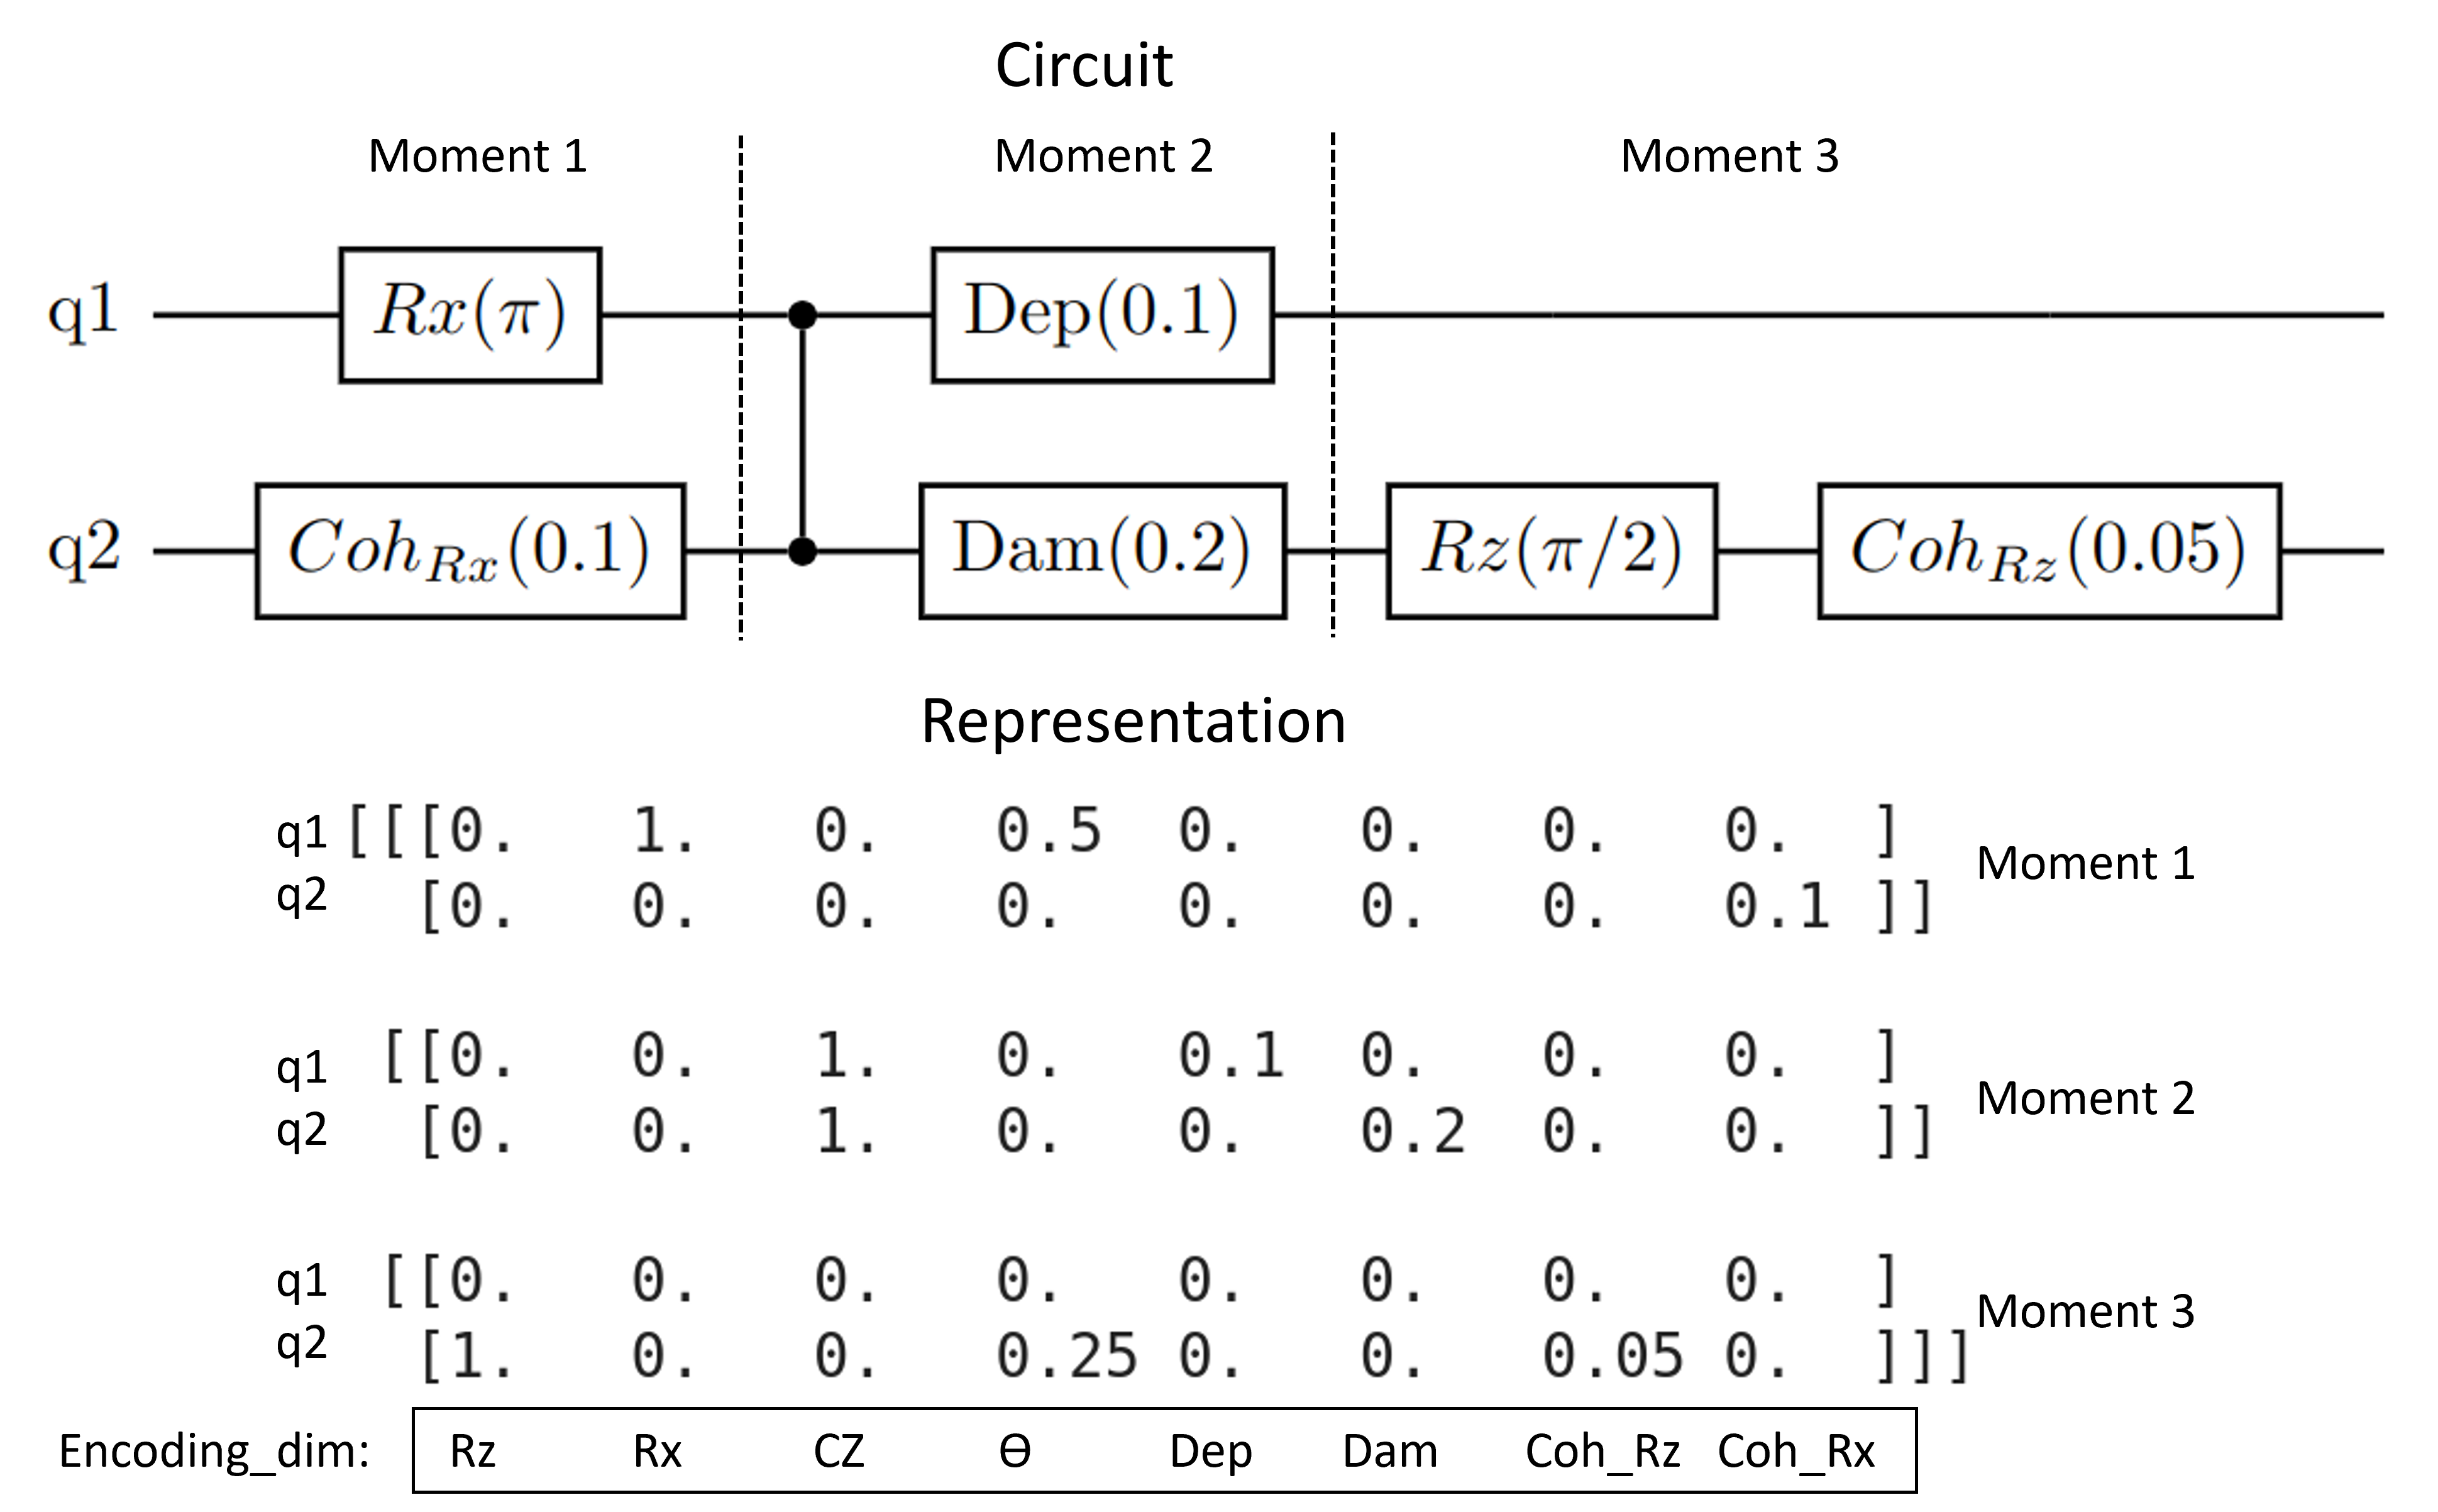
\includegraphics[width=0.49\textwidth]{circuit_representation.png}
    \caption{Example of the quantum circuit representation used in this work for a two-qubit quantum circuit.}\label{fig_qcr}
\end{figure}

\section{Results} \label{sec_results}
This section presents the results achieved using the proposed algorithm, both on simulations and on quantum hardware. 
A comprehensive description of the datasets utilized to derive these results is also provided.

\subsection{Dataset Generation}\label{sec_dataset}
In order to train a RL algorithm it is necessary to generate train, test and evaluation datasets.
All these datasets are composed of ensembles of random quantum circuits with their relative Density Matrices (DM). 
DMs are used as ground truth labels during the training of the algorithm (Section~\ref{sec_training}). 
DMs are analytically computed in simulations.  When circuits are executed on hardware, they can be extracted using quantum state 
tomography~\cite{PhysRevLett.109.120403}, or more efficient techniques like classical shadow state 
reconstruction~\cite{PRXQuantum.2.010307, Eisert_2020, PRXQuantum.2.030348}.\\ 
For the training and test sets, circuits have been generated with a fixed number of moments. 
A moment is a collection of gates that can be executed in parallel. The total number of moments in a quantum circuit is called depth.  
The evaluation datasets, used for performance benchmarking, are composed of circuits with different depths. 
For the datasets used for simulations it is possible to define a custom noise model, this will be described with accuracy in Section~\ref{sec_simulation}. 
All the datasets circuits have been generated by extracting random Clifford gates from among all the natives gates. 
We have used Clifford gates because of their good properties related to randomized benchmarking and shadow state estimation~\cite{2019npj, PhysRevA.77.012307, Eisert_2020, PRXQuantum.2.030348}.
The natives gates set is hardware specific and is composed of all gates that can be executed directly on hardware. 
For example, for this work, we have used the natives gates set of the Technology Innovation Institute (TII) quantum hardware, 
composed of $R_x$, $R_z$ and $CZ$ gates\footnote{TII quantum hardware uses $R_z$ and $GPI2$ as single qubit native gates. 
However, this last gate is equal to $R_x(\pi/2)$.}. It is important to notice that $R_x$ and $R_z$ are Clifford gates only when the rotation parameter 
is a multiple of $\pi/2$. We have also performed some preliminary tests with the IBM quantum hardware natives gates set~\cite{Santos_2016}, 
that uses the $CNOT$ gate as the two-qubits interaction native gate. Changing the natives gates is an easy procedure in the proposed algorithm 
and has not shown any significant performance change.

%% Copylot improved version
% \subsection{Dataset Generation}\label{sec_dataset}
% The training, testing, and evaluation datasets necessary for the Reinforcement Learning (RL) algorithm consist of ensembles of random quantum circuits and 
% their corresponding Density Matrices (DMs). These DMs serve as ground truth labels during the algorithm's training phase (Section~\ref{sec_training}). 

% In simulations, DMs are computed analytically. For circuits executed on hardware, DMs can be extracted using quantum state 
% tomography~\cite{PhysRevLett.109.120403} or more efficient techniques like classical shadow state 
% reconstruction~\cite{PRXQuantum.2.010307, Eisert_2020, PRXQuantum.2.030348}. 

% The training and test sets comprise circuits with a fixed number of moments, a term referring to a collection of gates that can be executed in parallel. 
% The total number of moments in a quantum circuit is its depth. Evaluation datasets, used for performance benchmarking, 
% consist of circuits with varying depths. 

% For the datasets used in simulations, a custom noise model can be defined, as detailed in Section~\ref{sec_simulation}. 
% All dataset circuits are generated by randomly extracting Clifford gates from the set of native gates, chosen for their beneficial 
% properties related to randomized benchmarking and shadow state estimation~\cite{2019npj, PhysRevA.77.012307, Eisert_2020, PRXQuantum.2.030348}. 

% The native gates set, which is hardware-specific, includes all gates that can be directly executed on the hardware. 
% In this work, we used the native gates set of the Technology Innovation Institute (TII) quantum hardware, 
% comprising $R_x$, $R_z$, and $CZ$ gates\footnote{TII quantum hardware uses $R_z$ and $GPI2$ as single qubit native gates. 
% However, the latter is equivalent to $R_x(\pi/2)$.}. Note that $R_x$ and $R_z$ are Clifford gates only when the rotation parameter is a multiple of $\pi/2$. 

% Preliminary tests were also conducted with the IBM quantum hardware native gates set~\cite{Santos_2016}, which uses the $CNOT$ gate as 
% the two-qubit interaction native gate. Changing the native gates is a straightforward procedure in the proposed algorithm and has 
% not shown any significant performance change.

\subsection{Simulations} \label{sec_simulation}

\begin{figure*}
    \centering
    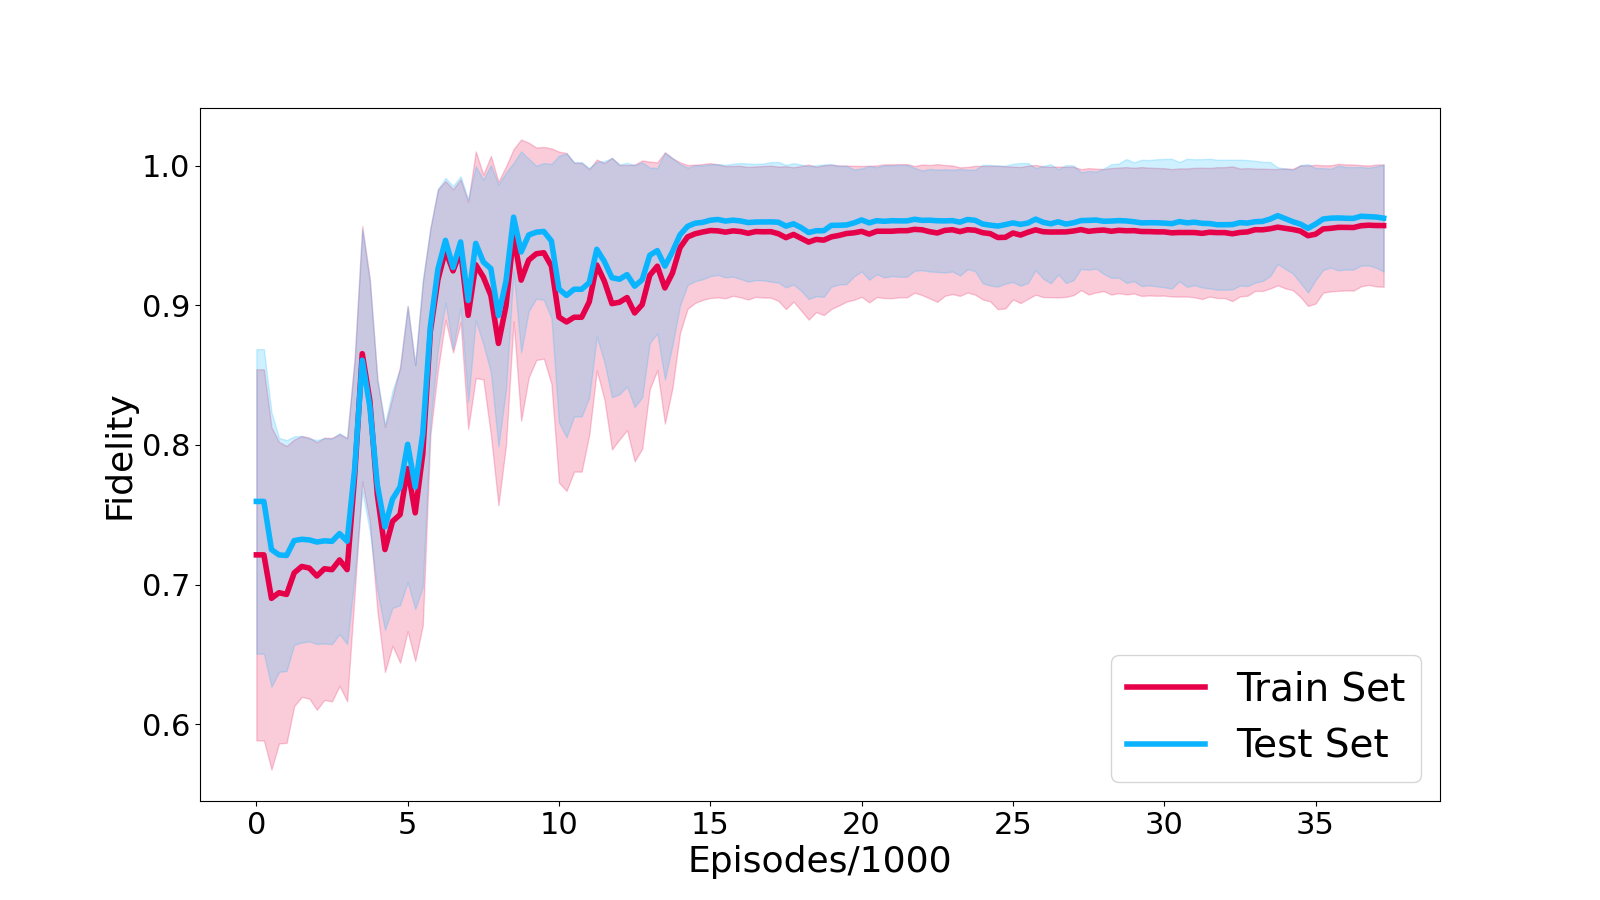
\includegraphics[width=\textwidth]{1Q_train_results.png}
    \caption{Average density matrix fidelity during training for single qubit circuits with simulated 
    custom noise model. Error bars represent the standard deviation.}\label{fig_1q_sim_train}
    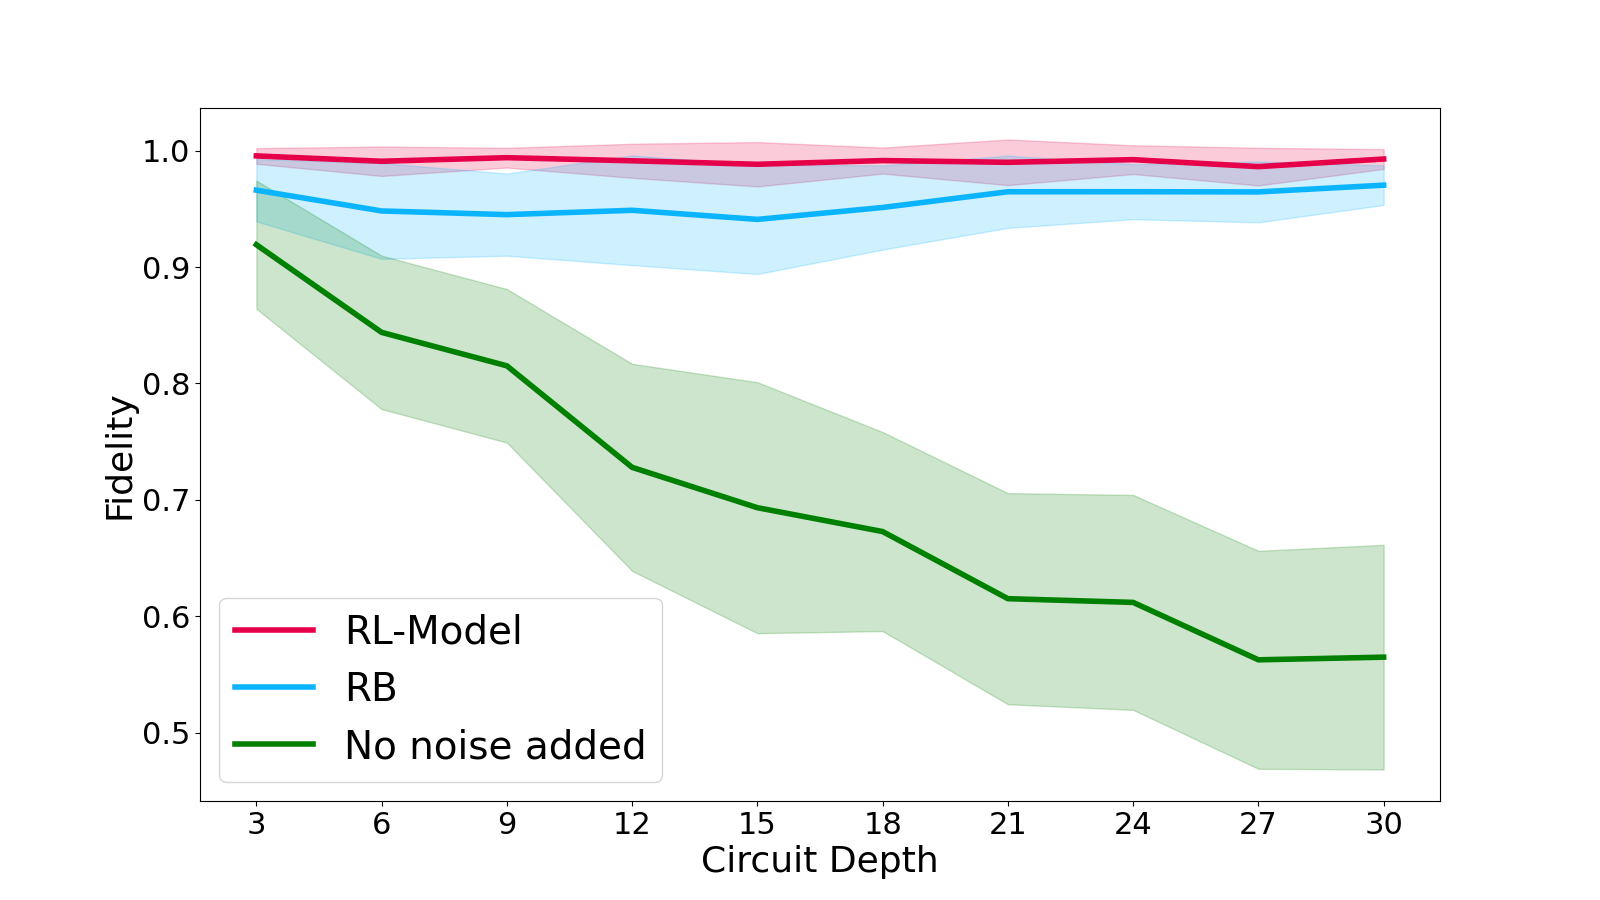
\includegraphics[width=\textwidth]{1Q_rb.png}
    \caption{Performance comparison of the RL agent with respect to the RB and the result obtained 
    without adding any noise channel. Error bars represent the standard deviation.}\label{fig_1q_sim_bench}
\end{figure*}

\begin{figure*}
    \centering
    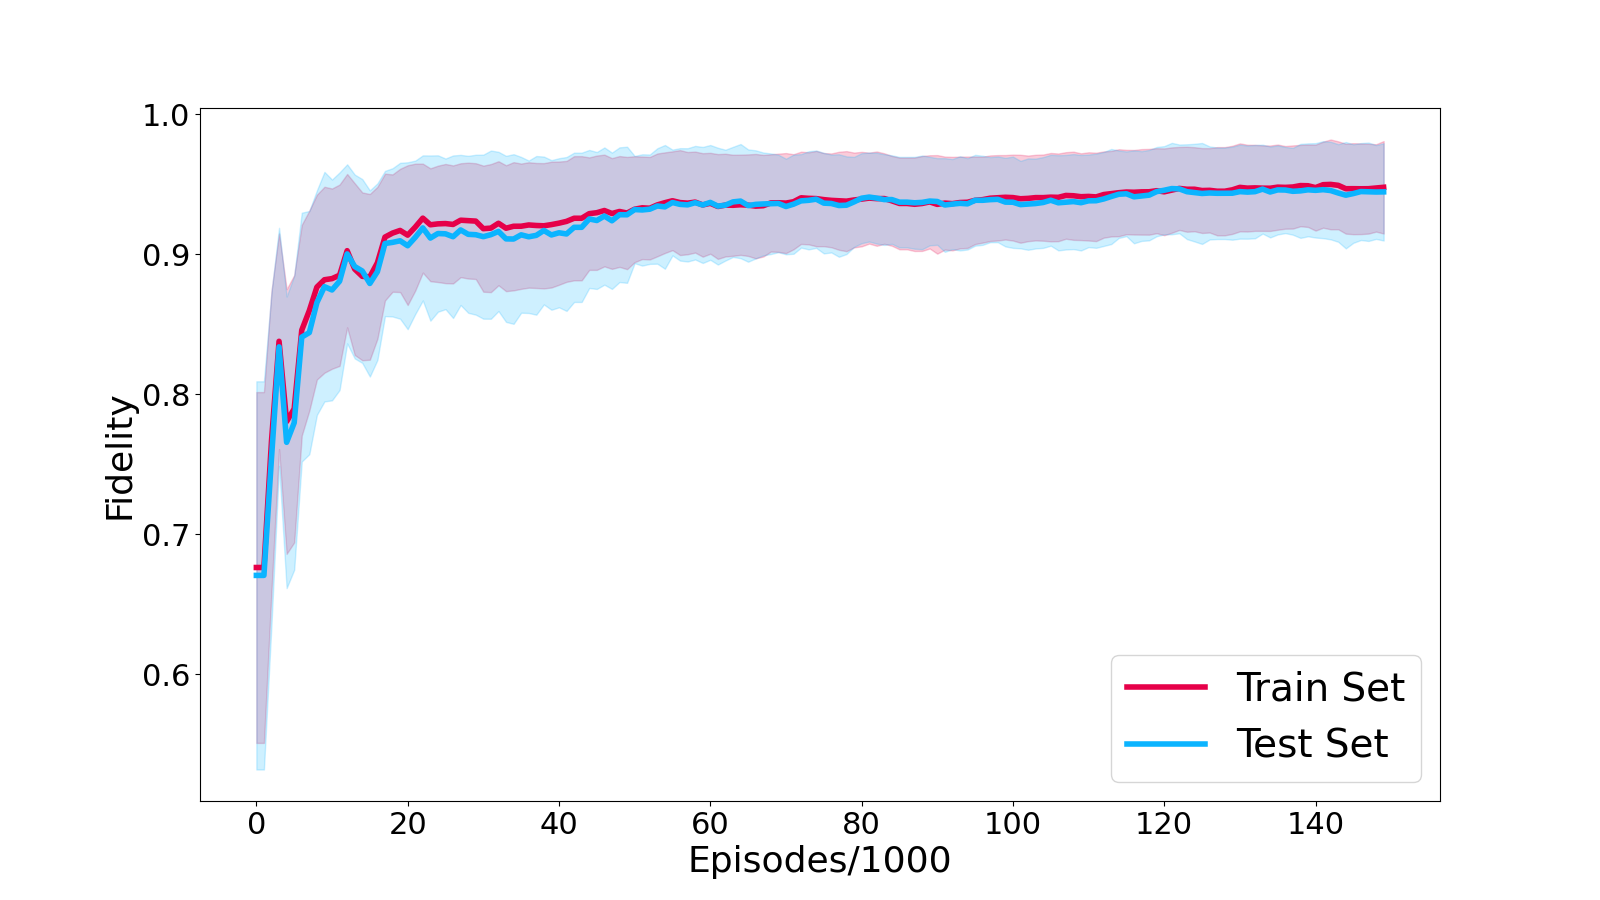
\includegraphics[width=\textwidth]{3Q_train_results.png}
    \caption{Average density matrix fidelity during training for three qubits circuits with simulated 
    custom noise model. Error bars represent the standard deviation.}\label{fig_3q_sim_train}
    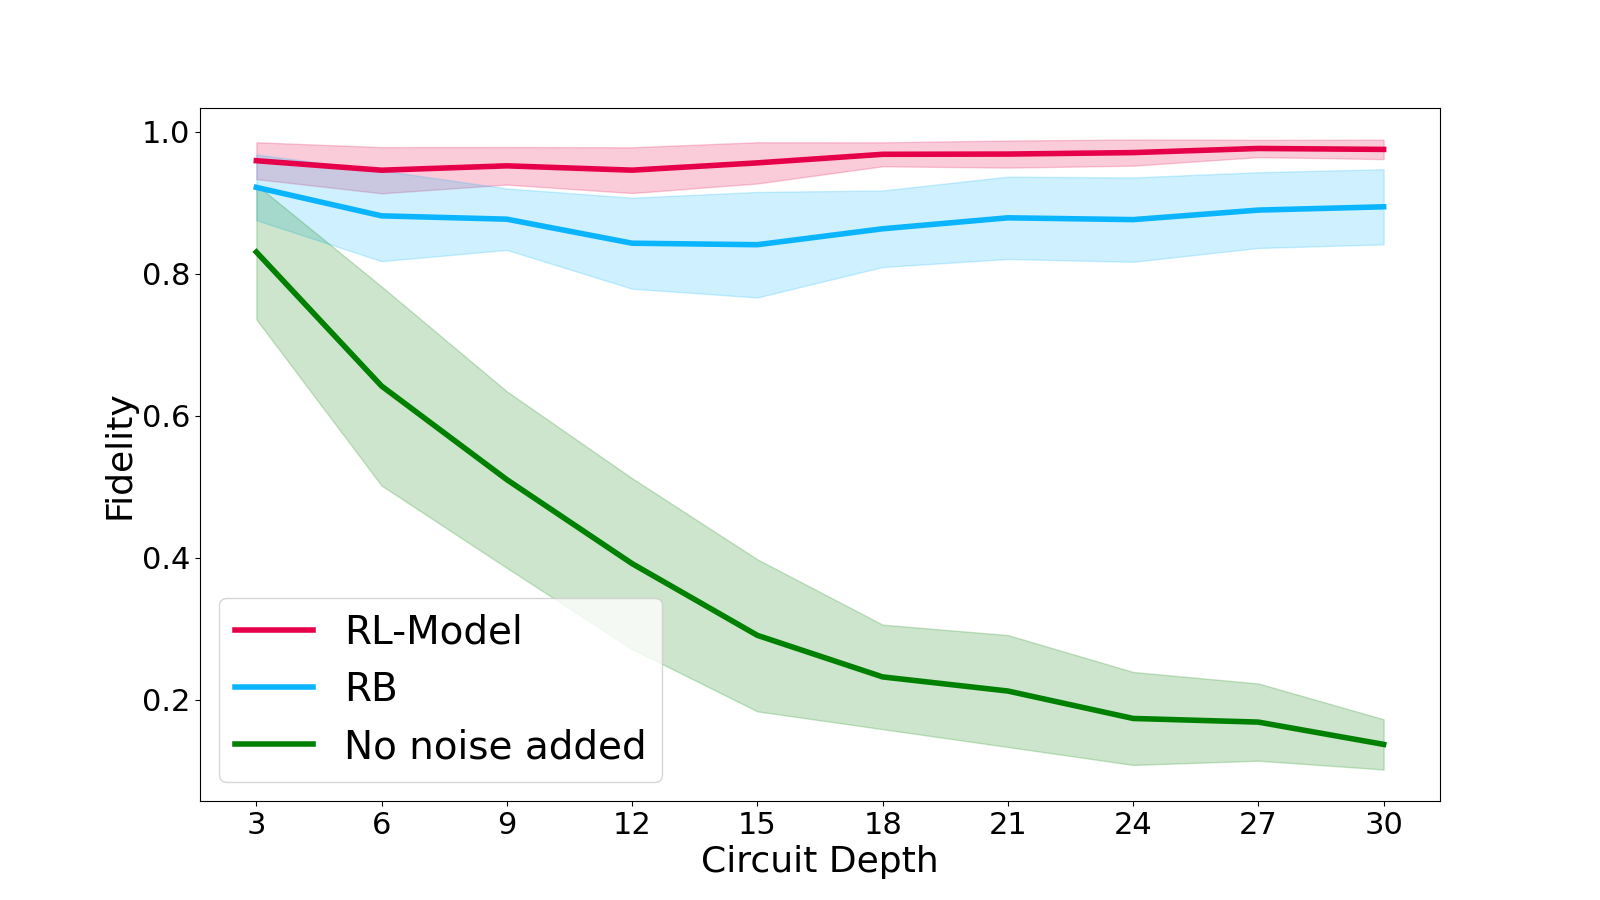
\includegraphics[width=\textwidth]{3Q_rb.png}
    \caption{Performance comparison of the RL agent with respect to the RB and the result obtained 
    without adding any noise channel. Error bars represent the standard deviation.}\label{fig_3q_sim_bench}
\end{figure*}

The first simulation involves single qubit circuits with a custom noise model. The parameters are as follows \TODO{Add table}:
A depolarizing channel with depolarizing parameter $0.1$ is applied after each $R_z$ gate.\\
An amplitude damping channel with decay parameter $0.05$ is applied after each $R_x$ gate.\\
A coherent $R_x$ error is applied after each $R_x$ gate. The parameter of the coherent error rotation 
($\theta^{'}$) depends on the gate rotation angle ($\theta$) as: $\theta^{'}=0.15\times\theta$.\\
A coherent $R_z$ error is applied after each $R_z$ gate. Also in this case, the parameter of the coherent 
error ($\theta^{'}$) depends on the $R_z$ rotation angle ($\theta$) as: $\theta^{'}=0.1\times\theta$.\\
This noise model is not meant to be realistic. Its purpose is to test the proposed algorithm on a noise model 
that depends on the gates types and the rotation parameters.\\
To train the RL agent, 500 random circuits of depth 7 were generated: 400 circuits for the training set and 
100 for the test set. Figure~\ref{fig_1q_sim_train} reports the average fidelity between DM as a function of 
the episodes, evaluated on both the training and test set. The standard deviation over our train and test sets 
is represented by error bars. The agent is able to learn the simulated noise, no overfit is observed. 
Convergence is reached after about $1.5\cdot10^5$ episodes, when the standard deviation of the fidelity begins 
to shrink.\\

\noindent
To test the model's generalization properties, we evaluated it on random circuits of varying lengths. 
Figure~\ref{fig_1q_sim_bench} shows the performance of the trained RL agent on circuits with depths ranging from 3 to 30. 
The RL agent was compared with the RB and the limit case where no noise channels were added to the circuits.\\
To use the RB as a noise predictor, we first extracted the decay parameter using the standard RB procedure. 
We then added a depolarizing channel with a depolarizing error equal to the decay parameter after each gate.\\
The RL agent can generalize to both longer and shorter circuits and consistently provides more accurate results than RB. 
This suggests that while RB treats all noise sources as depolarizing, our algorithm can identify the specific features of the noise. 
The improvement is especially noticeable on shorter circuits, as with larger depth, the noise can be approximated to a global depolarizing channel.\\

\noindent
We performed a similar simulation to test the proposed algorithm on circuits with multiple qubits. 
In the noise model, we slightly reduced the parameters of the coherent errors and added a depolarizing 
channel with a depolarizing error of $0.02$ and an amplitude damping channel with a parameter of $0.08$ 
after each $CZ$ gate. \TODO{Add table}\\
We generated a training set composed of 500 random three-qubit circuits of depth 7, with 400 circuits 
for training and 100 circuits for testing. Figure~\ref{fig_3q_sim_train} shows the average density matrix 
fidelity during training, with the standard deviation represented by error bars.\\
In this case, the algorithm can learn the noise, but convergence is much slower compared to single qubit 
circuits due to a larger action space that requires more episodes to be explored. Convergence is reached 
after about $5\cdot10^6$ episodes, with no overfit observed during the training process.\\
We compared the performance of the RL agent with RB and with the results obtained without adding noise for 
circuits of different lengths, as previously described for single qubit circuits (Fig.~\ref{fig_3q_sim_bench}). 
Again, the RL agent can generalize to circuits of different lengths and consistently provides more accurate 
results compared to RB.

\subsection{Quantum hardware}\label{sec_hardware}

\begin{figure*}
    \centering
    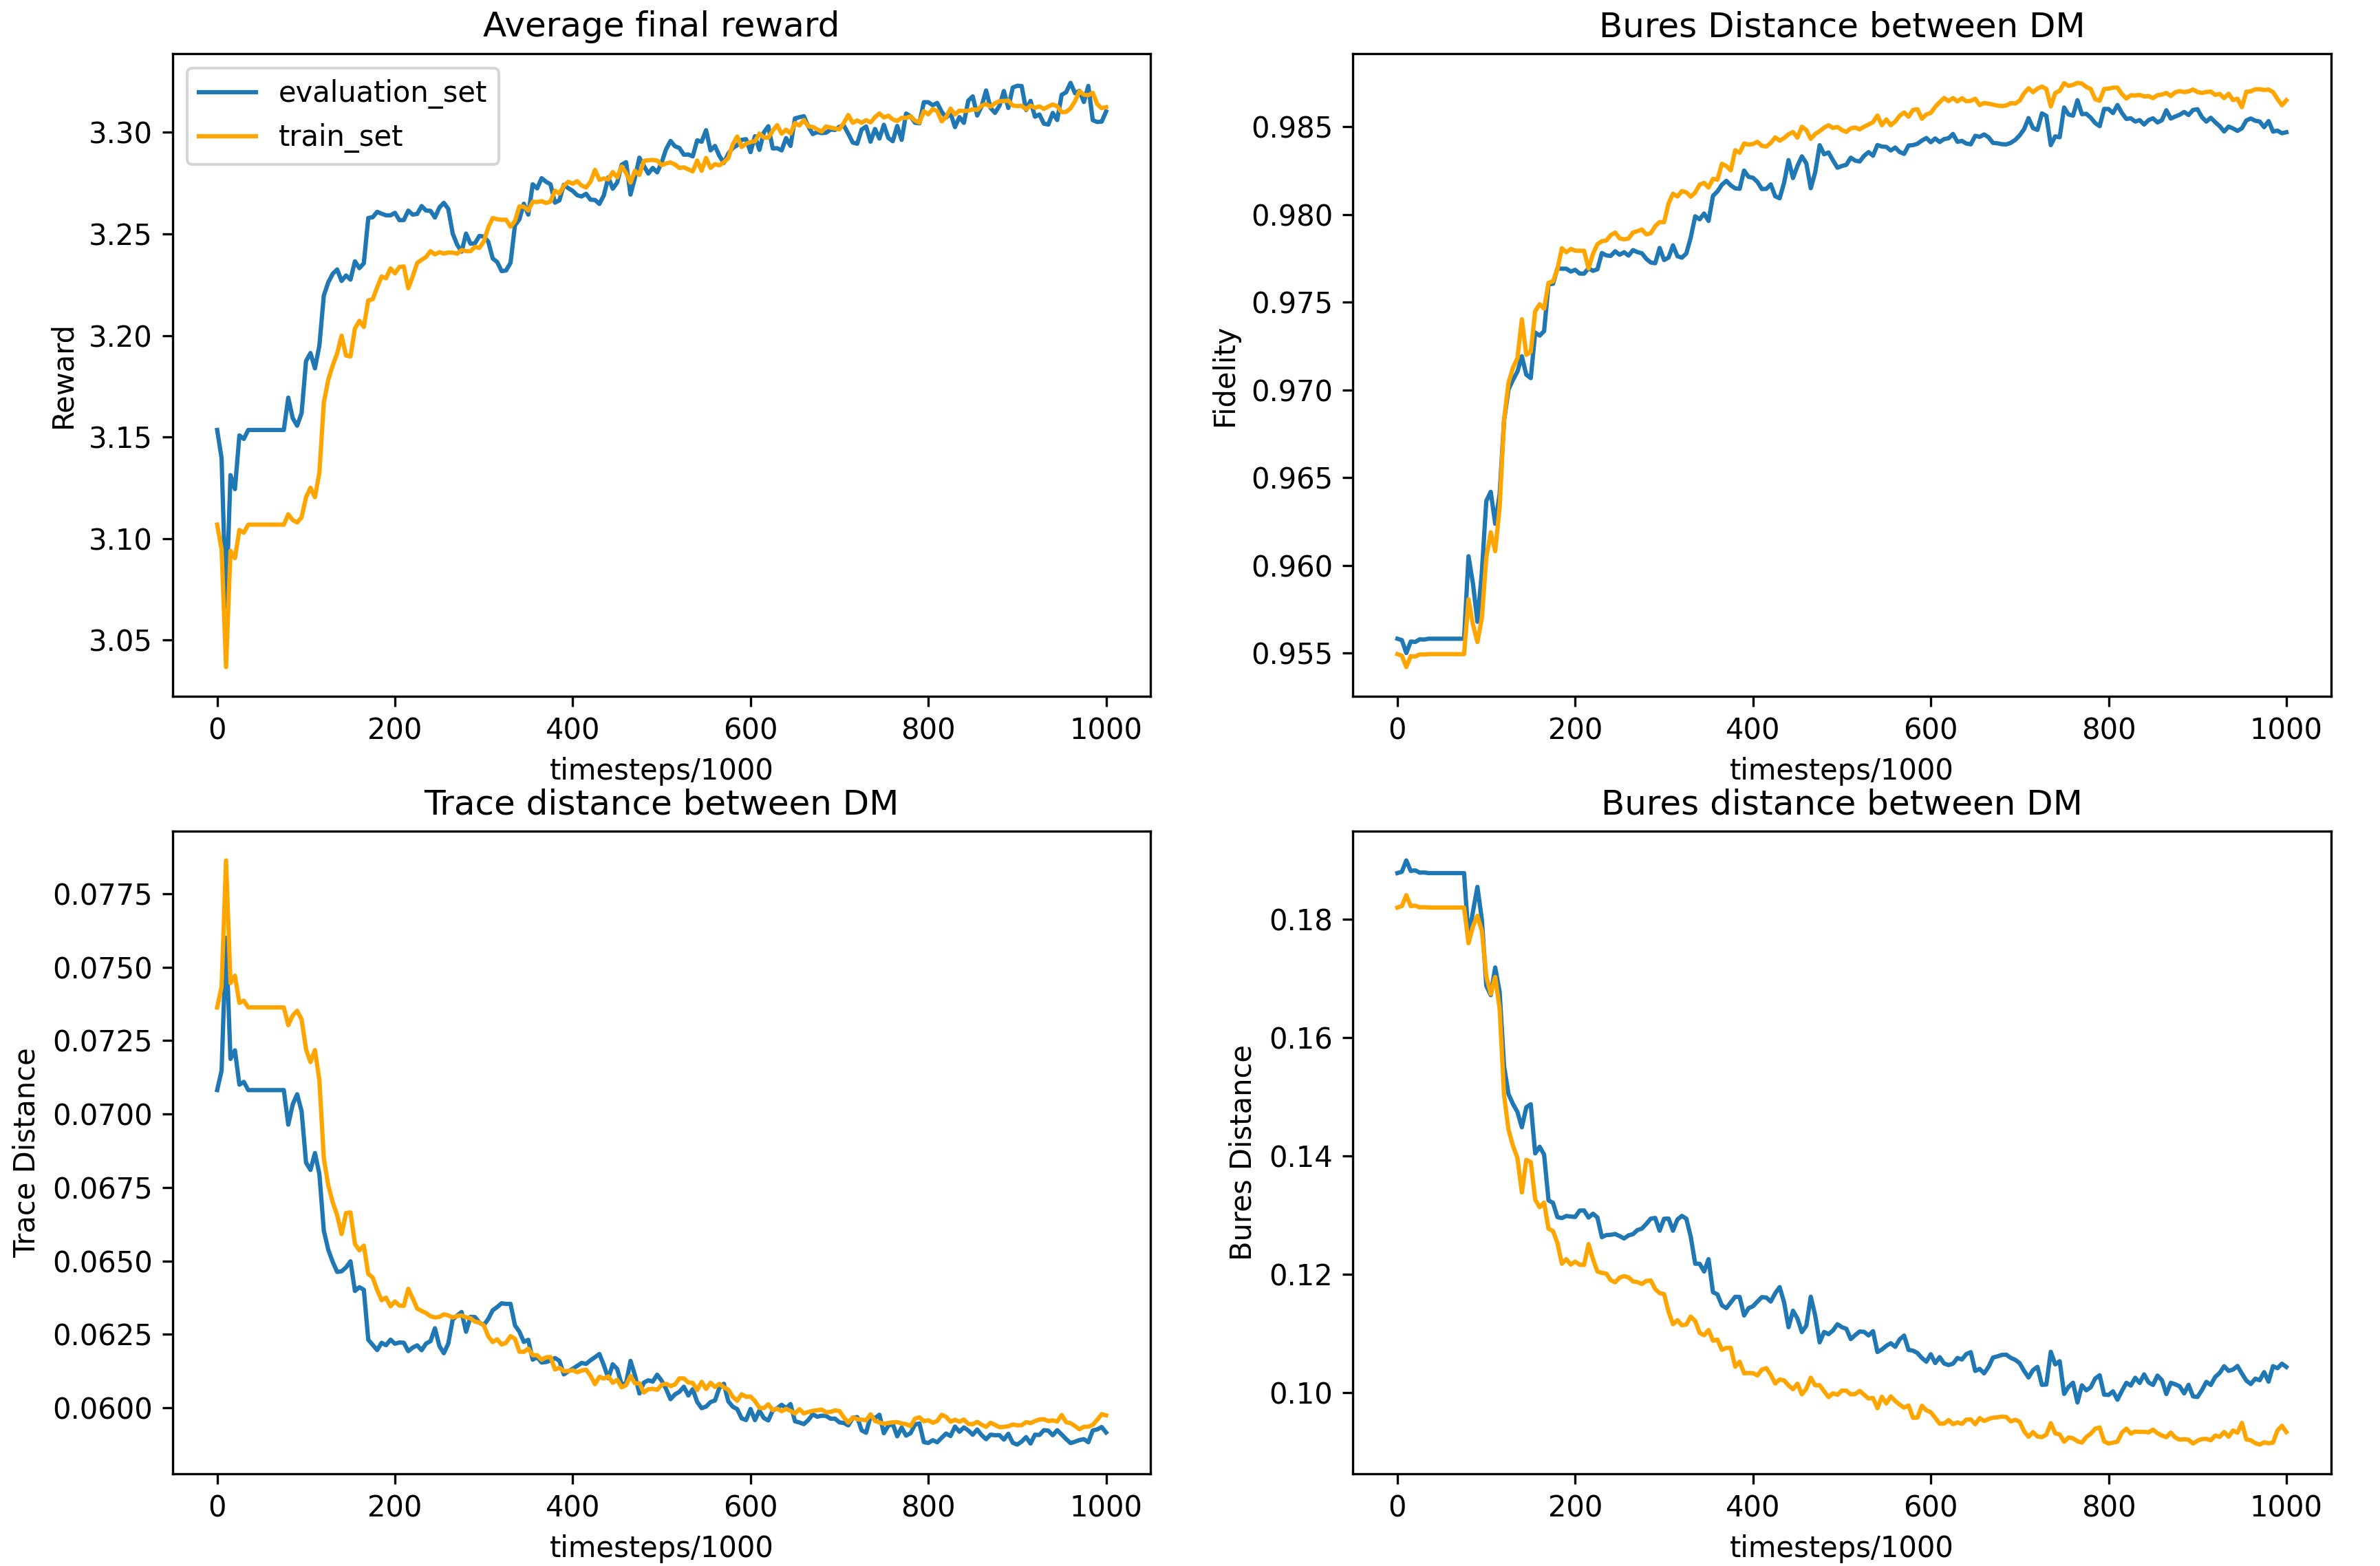
\includegraphics[width=0.6\textwidth]{training_hardware_1q.png}
    \caption{Average final reward and other evaluation metrics during training for one qubit circuits 
    executed on quantum hardware.}\label{fig_1q_hard_train}
    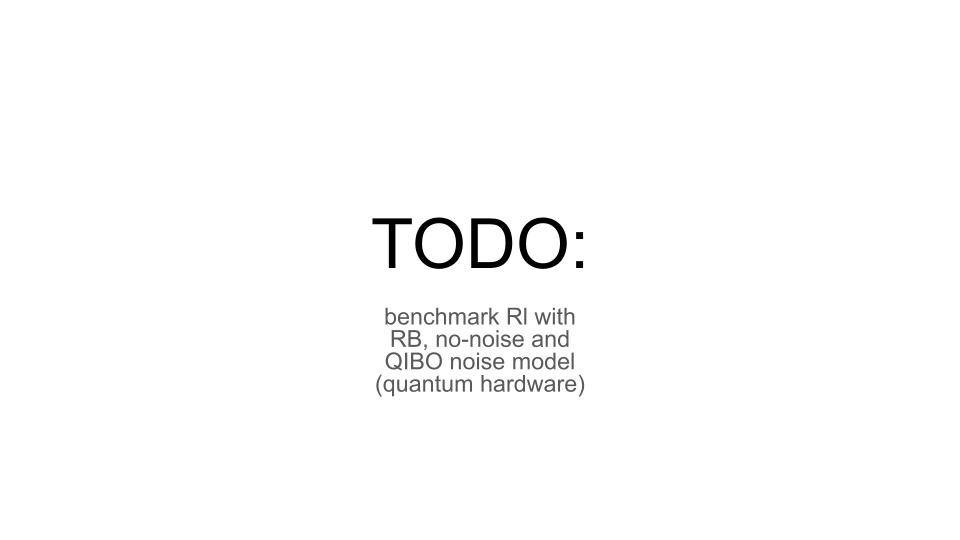
\includegraphics[width=0.6\textwidth]{benchmark_hardware_1q.png}
    \caption{Performance comparison of the RL agent with respect to the RB and the result obtained 
    without adding any noise channel. The performance has been computed using different metrics and 
    for circuits of different depth.}\label{fig_1q_hard_bench}
\end{figure*}

We tested the proposed algorithm on the quantum hardware of the Technology Innovation Institute of Abu Dhabi, 
using a single qubit superconducting transmon chip~\cite{doi:10.1126/science.1231930}. The dataset consists 
of 500 random circuits of depth 5, with 20\% used as the test set. 

To compute the DMs of the circuits, we used state tomography. For more accurate DMs, we applied the readout 
error mitigation technique. The fidelity between the DMs of perfect circuits and those executed on hardware 
averages 0.95, suggesting minimal noise accumulation during circuit execution. This is a different condition 
compared to the simulations where a lot of noise was added to the circuits. 

Figure~\ref{fig_1q_hard_train} reports average final reward and other evaluation metrics during training. 
The performance benchmarking of the RL agent was performed as described in Section~\ref{sec_simulation}. 
Figure~\ref{fig_1q_hard_bench} reports the performance of the trained agent compared with RB, QIBO built-in 
noise model, and the circuits without noise.
\newpage
\section{Applications} \label{sec_applications}
In this section we report two example applications of the proposed algorithm. The first application has been performed on simulations and studies the results obtained with a Quantum Fourier Transform (QFT) circuit and Grover's algorithm circuit. The second example regards an application to quantum machine learning and has been performed on TII quantum hardware. These tests are helpful to study the generalization properties of the proposed model and offer a solid stress test and benchmarking of the overall performance.

\subsection{Quantum algorithms}
We tested the proposed model on two well-known quantum algorithms: the Quantum Fourier Transform (QFT) 
\cite{Shor_1997} and Grover's search algorithm \cite{grover1996fast}. We used simple cases of these 
algorithms to work with relatively small quantum circuits.\\
For the QFT algorithm, we did not insert SWAP gates at the end of the circuit to reverse the qubit order. 
Grover's algorithm uses one ancillary qubit, and the search target state is $\ket{11}$. This setup requires only 
one oracle call to find the target state.\\
In both cases, the circuits consist of three qubits. We used the same noise model described in 
Section~\ref{sec_simulation}. We transpiled the circuits to use TII native gates ($R_z$, $R_x$, and $CZ$). 
After gate decomposition, we report the number of gates and other important circuit parameters in 
Table~\ref{tab_gates}.\\
These circuits have similar characteristics to those used in Section~\ref{sec_simulation} for comparison 
with RB, in terms of the number of gates and circuit moments. However, the fraction of $CZ$ gates differs. 
All training and testing circuits were generated randomly with equal probability for each gate type, 
resulting in about $1/3$ of $CZ$ gates.
Moreover, not all gates in the transpiled circuits are Clifford, as the parameters of $R_z$ and $R_x$ gates 
are not fixed multiples of $\pi/2$.

\begin{table}[ht]
\centering
\caption{Number of gates and circuit moments of the transpiled circuits for QFT and Grovers's algorithm.}
\label{tab_gates}
\begin{tabular}{@{}llll@{}}
\toprule
& Total gates & $CZ$ gates & Moments \\
\midrule
QFT & 53 & 6 & 37 \\
Grover & 40 & 7 & 25 \\
\bottomrule
\end{tabular}
\end{table}

\noindent
For both QFT and Grover's circuits, we compared the noise model of the RL agent trained in 
Section~\ref{sec_simulation} with the RB noise model. The depolarizing parameter for the RB model was 
obtained in Section~\ref{sec_simulation}. 
Table~\ref{tab_results} reports the fidelity between the reconstructed density matrix and the original 
noisy density matrix for both noise models. The RL agent outperforms the RB model, especially for the QFT 
circuit.

\begin{table}[ht]
\centering
\caption{Fidelity between the density matrix reconstructed with a noise model (RL agent or RB) and the original noisy one. 
The result is reported for both QFT and Grover's algorithm circuits.}
\label{tab_results}
\begin{tabular}{@{}lll@{}}
\toprule
& RL & RB \\
\midrule
QFT & 0.88 & 0.80 \\
Grover & 0.95 & 0.94 \\
\bottomrule
\end{tabular}
\end{table}

\begin{figure*}
    \centering
    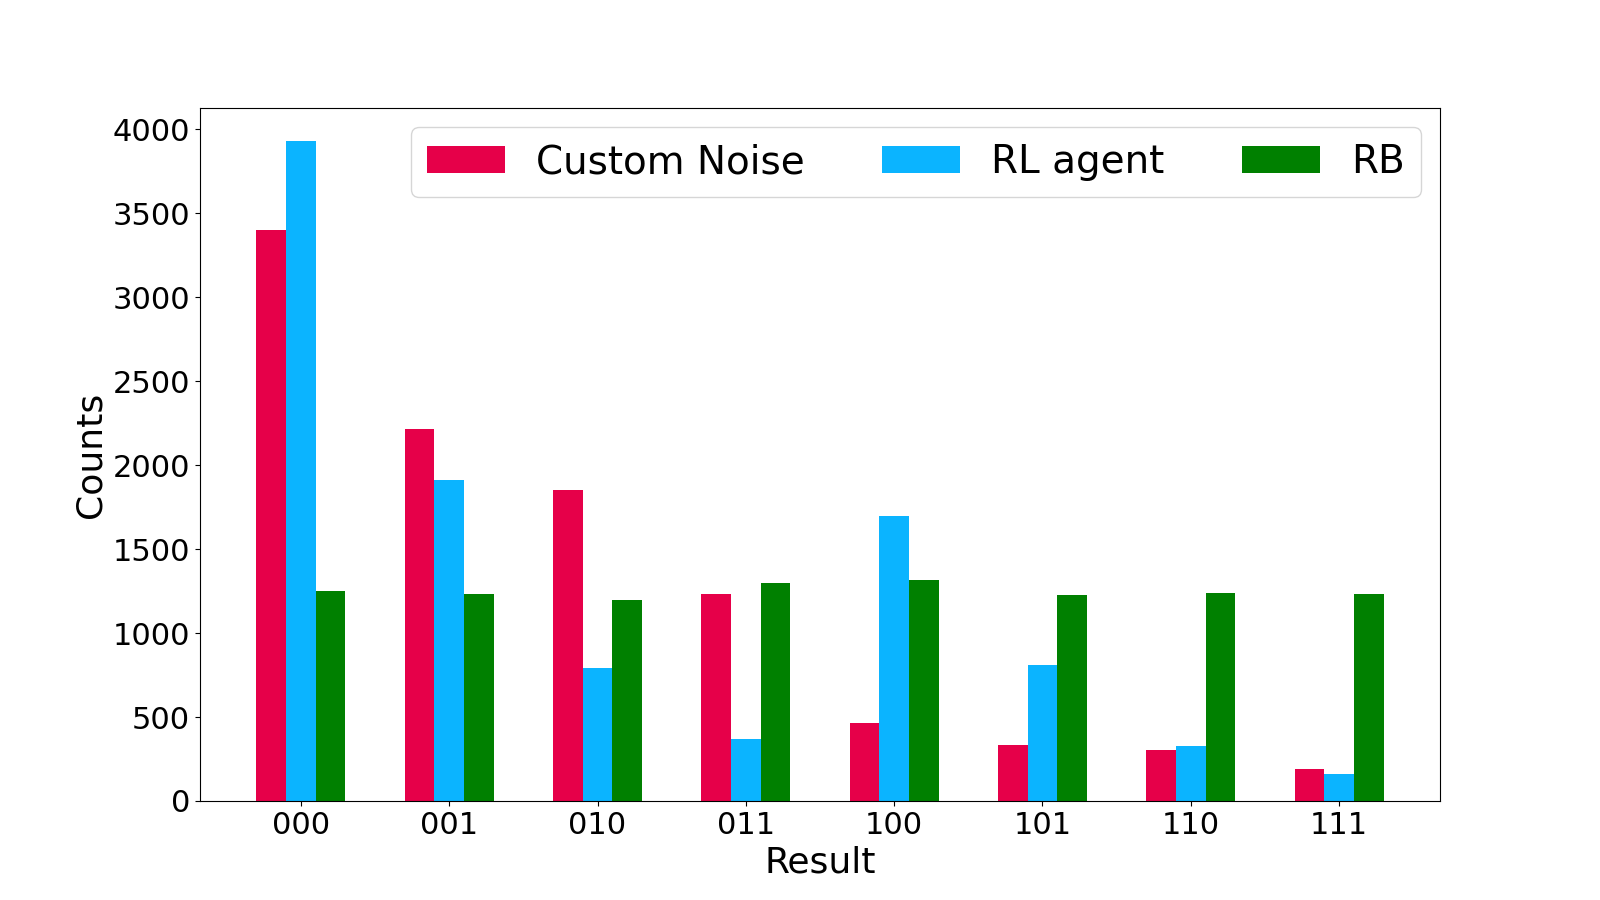
\includegraphics[width=\textwidth]{QFT_shots.png}
    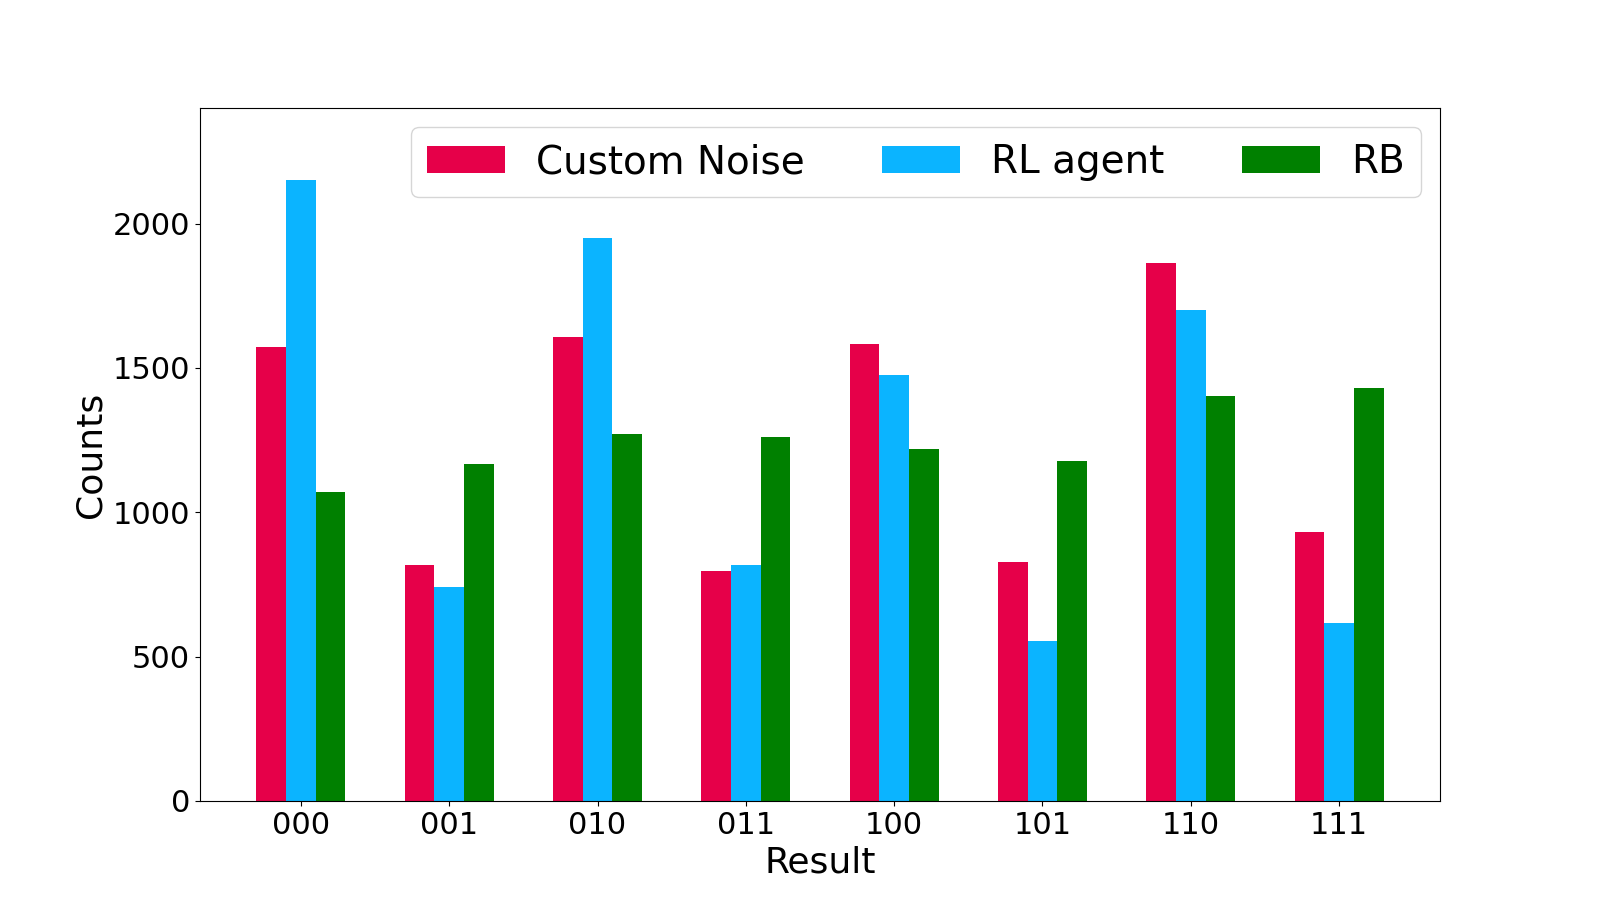
\includegraphics[width=\textwidth]{Grover_shots.png}
    \caption{Shots simulation for the three qubits QFT (top) and Grover's algorithm (bottom) quantum circuits. The histograms show a comparison between the counts obtained with the original custom noise model, the RL agent noise model and the RB noise model. For each noise model and circuit the simulation has been performed using $10^5$ shots.}\label{fig_algorithms}
\end{figure*}

\noindent
Figure~\ref{fig_algorithms} presents a circuit shots simulation performed with $10^5$ shots on both QFT 
and Grover's algorithm circuits. The histograms compare the counts obtained with the original noisy circuit 
and the reconstructed one using the RL agent and the RB noise model.\\
Given the length of the employed circuits, the RB noise model tends to average the output. Conversely, the RL 
agent can produce results that, with a few exceptions, align well with the shots obtained with the original 
noise model. This is particularly evident in the QFT simulation counts for the states $\ket{000}$ and 
$\ket{001}$. These states are the most measured due to the noise model (owing to the presence of amplitude 
damping channels), a feature clearly reproduced by the RL agent.\\
The results in this section demonstrate the proposed RL approach's strong generalization properties for noise 
modeling. It can adapt to circuits with a structure different from the random ones used in the training set 
and with significantly different lengths. Importantly, the algorithm showed no adaptation issues when tested 
on circuits containing some non-Clifford rotation gates.

\subsection{Quantum machine learning}

\section{Conclusions}
\todo{INCLUDE NEW RESULTS}
This work introduced a reinforcement learning (RL) algorithm for replicating specific noise models in 
single and multiple qubit quantum circuits. Our model outperformed the standard noise characterization 
method, randomized benchmarking, in both simulation and quantum hardware execution.\\
The RL model's future applications include noise characterization within quantum circuits. By learning 
the error patterns of qubits for specific gate types, the model could optimize the transpilation process 
\cite{9259930}, thereby enhancing algorithm fidelity. Furthermore, using the knowledge of the noise for 
its mitigation could be an interesting approach.\\
The current limitation of the model is its scalability to circuits with many qubits. To overcome this, 
we are considering potential solutions. One approach could involve training the model with probability 
distributions derived from measurements instead of density matrices. Another solution could be partitioning 
into smaller circuits, enabling parallel training of multiple small models.\\
While these ideas are conceptual and require further theoretical validation, this work demonstrated that 
using machine learning to learn noise patterns within small quantum circuits is a promising proof of concept 
that could drive future advancements.

\backmatter

\section*{Declarations}

\textbf{Funding:} 
This work is partially supported by the Technology Innovation Institute (TII), Abu Dhabi, UAE.\\
This work is partially supported by ICSC – Centro Nazionale di Ricerca in High Performance Computing, 
Big Data and Quantum Computing, funded by European Union – NextGenerationEU.\\

\noindent
\textbf{Conflict of interest/Competing interests:}
Authors declare no conflict of interest.\\

\noindent
\textbf{Open access:}
Copyright for this paper by its authors. Use permitted under Creative Commons License Attribution 4.0 International (CC BY 4.0).\\

\noindent
\textbf{Data Availability:} Both the datasets and the code used for this study are available, on request, by contacting
the authors.\\

\noindent
\textbf{Author contribution:} 
S. Bordoni, A. Papaluca, P. Buttarini, A. Sopena: Methodology, Software, Writing.\\
S. Carrazza, S. Giagu: Project Administration, Review, Funding.\\


\bibliography{sn-bibliography}

\end{document}
